%% Overleaf			
%% Software Manual and Technical Document Template	
%% 									
%% This provides an example of a software manual created in Overleaf.

\documentclass{ol-softwaremanual}

% Packages used in this example
\usepackage{graphicx}  % for including images
\usepackage{microtype} % for typographical enhancements
\usepackage{minted}    % for code listings
\usepackage{amsmath}   % for equations and mathematics
\setminted{style=friendly,fontsize=\small}
\renewcommand{\listoflistingscaption}{List of Code Listings}
\usepackage{hyperref}  % for hyperlinks
\usepackage[a4paper,top=4.2cm,bottom=4.2cm,left=3.5cm,right=3.5cm]{geometry} % for setting page size and margins

% Custom macros used in this example document
\newcommand{\doclink}[2]{\href{#1}{#2}\footnote{\url{#1}}}
\newcommand{\cs}[1]{\texttt{\textbackslash #1}}

% Frontmatter data; appears on title page
\title{Supernova Bootcamp}
\version{0.0.0}
\author{Lauren Aldoroty}
%\softwarelogo{\includegraphics[width=8cm]{logo}}

\begin{document}

\maketitle

\tableofcontents
% \listoflistings
\newpage

\section{Introduction}

Compiling all the things I've learned so it's easier for future folks. This manual will attempt to cover more technical, data-analysis driven perspectives on working with SNe, particularly SNe Ia. In the Software section (Section~\ref{sec:software}), at the end of each subsection, I'll list some lesser-known functions and tricks that I've found useful. These will be indicated by section titles \texttt{in font like this}, e.g., \texttt{helio\_to\_cmb()} (Section~\ref{sec:heliotocmb}).

\section{Reddening and Extinction}

Reddening and extinction are \textit{nearly} the same thing, but not quite. They're both caused by light scattering off dust, but \textit{extinction} describes the dimming that results, and \textit{reddening} describes the preferential scattering of blue light (i.e., more shorter wavelength light gets scattered away from us than longer wavelengths, so we see objects as redder than they actually are.) This is important because it's a pretty large source of systematic uncertainty in supernova studies! Dust doesn't emit light, it just takes it away, so we can't ``see'' it directly. \textit{HOW} are we supposed to correct for an effect we know so little about? 

\subsection{Background}
Extinction, in general, is described by the equation:
\begin{equation}
    A_{V} = -2.5\log \frac{F_{V}}{F_{V,0}},
\end{equation}

where the subscript $V$ indicates the $V$-band photometric bandpass, $F_{V}$ is observed flux in the $V$-band, and $F_{V, 0}$ is the intrinsic flux in the $V$-band.

Reddening is described by:
\begin{equation}
    E(B-V) = (B-V)_{observed} - (B-V)_{intrinsic},
\end{equation}

where $(B-V)_{observed}$ is the observed $B-V$ photometric color, and $(B-V)_{intrinsic}$ is the intrinsic photometric color. Note that because magnitudes are logarithmic, this equation is a ratio, too! We can link extinction and reddening with an equation, as well:
\begin{equation}
    E(B-V) = A_{B} - A_{V},
\end{equation}

where $A_{B}$ is photometric extinction in the $B$-band and $A_{V}$ is photometric extinction in the $V$-band. We can also link them like this:
\begin{equation}
    A_{V} = R_{V}E(B-V),
\end{equation}

where $R_{V}$ is a constant called the ``total-to-selective extinction ratio''. Basically, it's a constant that tells you how much light you lose in a particular photometric band. 

\begin{figure}
    \centering
    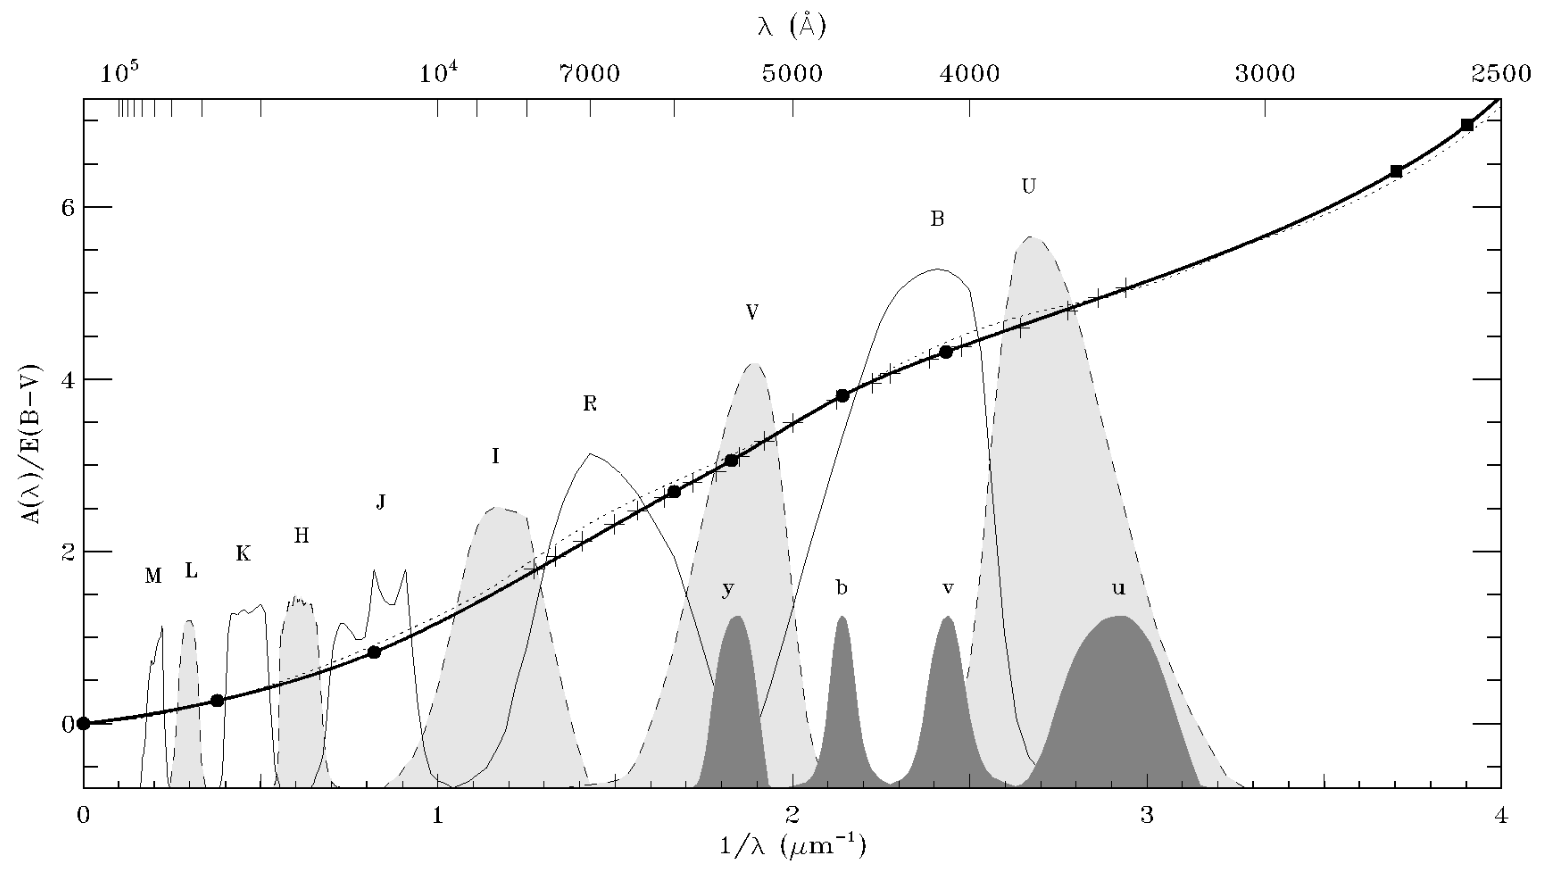
\includegraphics[width=0.99\textwidth]{figs/fitzpatrick1999.png}
    \caption{$R_{X}$ ($X$ for an arbitrary filter) for Johnson photometric filters (transmission functions shown scaled arbitrarily for reference). Solid points are data, the solid line is a cubic spline interpolation (\textit{not} a fit). Note that extinction has a more significant effect at shorter wavelengths. Figure from \cite{Fitzpatrick1999}.}
    \label{fig:phot_reddening}
\end{figure}

\subsection{Correcting for Dust}

There are a few packages you can use to quickly un-dust your data. First, \href{https://dust-extinction.readthedocs.io/en/stable/}{\texttt{dust\_extinction}} has a bunch of dust extinction curves and allows you to redden or deredden the spectrum by multiplying or dividing by the dust model's \texttt{extinguish} attribute, respectively. It also takes care of units for you, so you'll need \href{https://docs.astropy.org/en/stable/units/index.html}{\texttt{astropy}'s \texttt{units} module}. You have to provide it with $E(B-V)$ or $A_{V}$ as well. I like to get that with the SNooPy \texttt{get\_dust\_RADEC()} function, which retrieves the Milky Way $E(B-V)$ from \href{https://irsa.ipac.caltech.edu/frontpage/}{IRSA} based on RA and Dec (Section~\ref{sec:snpydustfuncs}). Here's some pseudocode showing how I deredden the flux for a spectrum:

\begin{minted}[
    bgcolor=lightgray,
    frame=leftline,
    framesep=-3mm]
    {python}

    from astropy import units as u
    from dust_extinction.parameter_averages import F04
    from snpy.utils.IRSA_dust_getval import get_dust_RADEC

    dustmodel = F04(Rv=3.1)
    mwreddening = get_dust_RADEC(ra, dec, calibration='SF11')[0][0]
    dereddened_flux = ((flux*u.erg/(u.s*u.AA*u.cm**2))/
        dustmodel.extinguish(wave*u.AA, Ebv=mwreddening)).value
    
\end{minted}
\section{Hubble's Law and SN Ia Cosmology}

\subsection{What the heck is a rest frame?}

Let's say you have some data, but it's from a supernova with $z = 0.1$. Because of the relativistic Doppler effect, the wavelengths you \textit{observe} are different from the ``actual'' wavelengths, i.e., rest frame wavelengths. This will also affect observed flux. Ignoring ejecta velocity (see Section \ref{sec:ejectavelocity}), this is why a spectral line won't appear in its ``expected'', or rest frame, position. Usually, you want to put your spectra in the rest frame before doing anything with them because it's hard to compare SNe at different redshifts. See Section~\ref{sec:spec_restframe} for details on correcting SN spectra to the rest frame. 

\subsection{$z_{helio}$ and $z_{CMB}$}

You'll encounter two kinds of redshift---heliocentric redshift ($z_{helio}$) and CMB (Cosmic Microwave Background) redshift ($z_{CMB}$). \textit{These are different, and are used for different purposes!} $z_{CMB}$ is the redshift caused by the Universe's expansion \textit{only}, i.e., where the reference frame is the CMB frame. $z_{helio}$ is the redshift with \textit{only} the Earth's rotation and orbit removed. There are still effects from other motion, like Galactic rotation and the Galaxy moving around with respect to other objects, as well as $z_{CMB}$. ``Heliocentric'' $\equiv$ ``Sun at center'', so ``Sun at center'' is the rest frame. It's how things are moving relative to the Milky Way. Note that $z_{helio}$, while often reported as an object's redshift, is \textit{not} the observed redshfit. The observed redshift does not have the Earth's rotation and orbit removed. In other words, $z_{helio}$ contains information about a bunch of things moving relative to each other, including motion relative to the CMB, while $z_{CMB}$ contains information about \textit{only} motion relative to the CMB.

For cosmology, you'll use $z_{CMB}$ (e.e., when making a Hubble diagram or determining other cosmological parameters). If you're dealing with data that you need to correct to the rest frame, you probably want to use $z_{helio}$.

\subsection{How to make a Hubble diagram}
Firstly, what is a Hubble diagram? It's a plot of recession velocity ($y$-axis) vs. distance ($x$-axis) (Figure \ref{fig:oghubble}). Turns out these things are positively correlated. In plain English, the farther away a galaxy is, the faster it's hurtling away from us (and everything else---the Universe is homogeneous and isotropic). This means the Universe is expanding\footnote{It's expanding at an accelerating rate, but this statement and a very crude Hubble diagram alone do not imply accelerated expansion}!

\begin{figure}[h!]
    \centering
    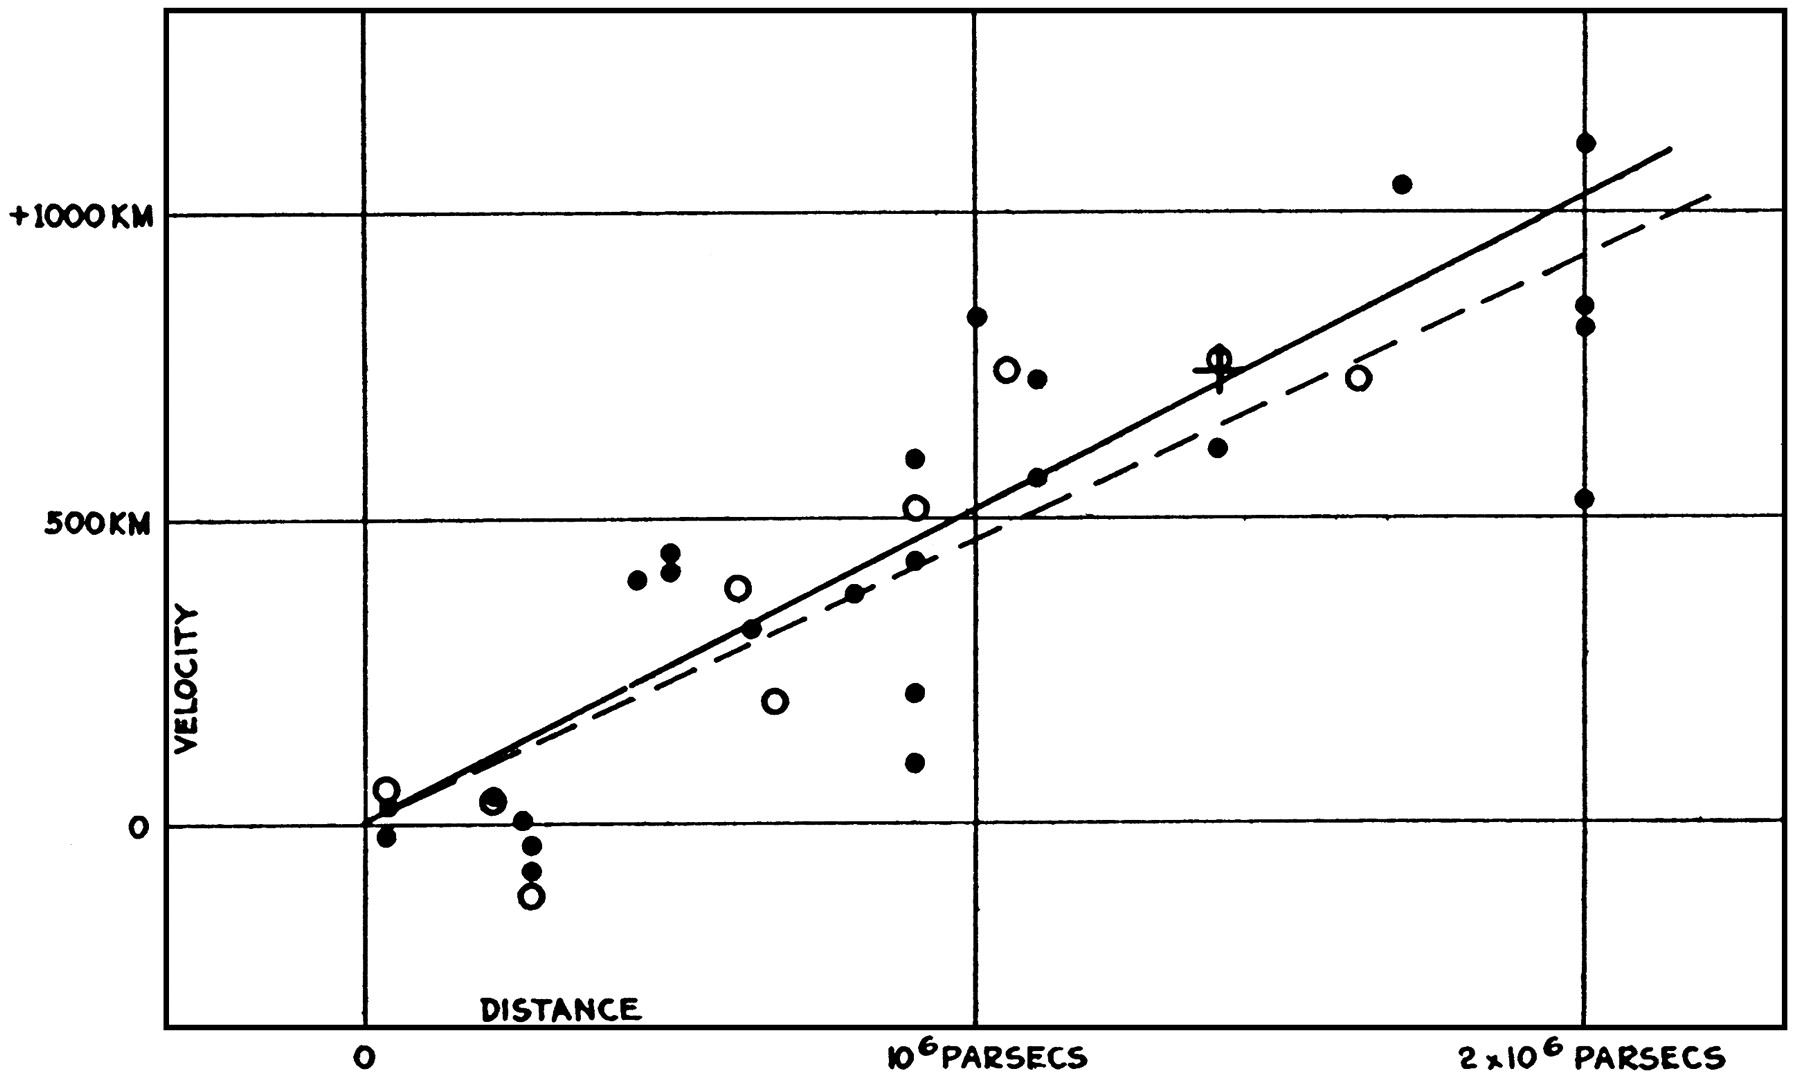
\includegraphics[width=0.7\textwidth]{figs/hubble_diagram_og.jpeg}
    \caption{The OG Hubble diagram. Note that the velocity units are km---\textit{this is a mistake}. It should probably be km/s. Even Edwin Hubble made an error on his most famous published figure. You're doing just fine.}
    \label{fig:oghubble}
\end{figure}

However, no one really uses linear distance units, like parsecs, or velocities like parsecs per second in Hubble diagrams in the literature any more. You still might see these, though. Units you may see to represent recession velocity on the $y$-axis include:
\begin{itemize}
    \item km/s
    \item The distance modulus $\mu$ (apparent magnitude minus absolute magnitude, $m-M$.)
\end{itemize}
Units you may see to represent distance on the $x$-axis include:
\begin{itemize}
    \item Mpc
    \item $z$
    \item log($z$) or log($cz$)
\end{itemize}
You'll most commonly see the distance modulus. It's the difference between apparent magnitude, $m$, and absolute magnitude, $M$. So, if the difference between these quantities is large, then an object is further away. If the difference is small, it's closer. You can think of $M$ as the intrinsic brightness of an object. $m$ is the brightness that you observe, corrected for effects like dust extinction (and because we're supernova people, also stuff like the luminosity-decline rate relation). 

So, there are many ways you can actually make a Hubble diagram because there are a zillion ways to standardize SNe Ia. Let's discuss using $\chi^{2}$ minimization. 

\subsection{Hubble residual}
The Hubble residual is the difference between the observed distance modulus of an SN and the expected distance modulus, obtained by fitting a cosmology to the data. This is important because this quantifies the uncertainty in our cosmological parameters. So, a lot of work is centered around minimizing the Hubble residual. 

\begin{figure}[h!]
    \centering
    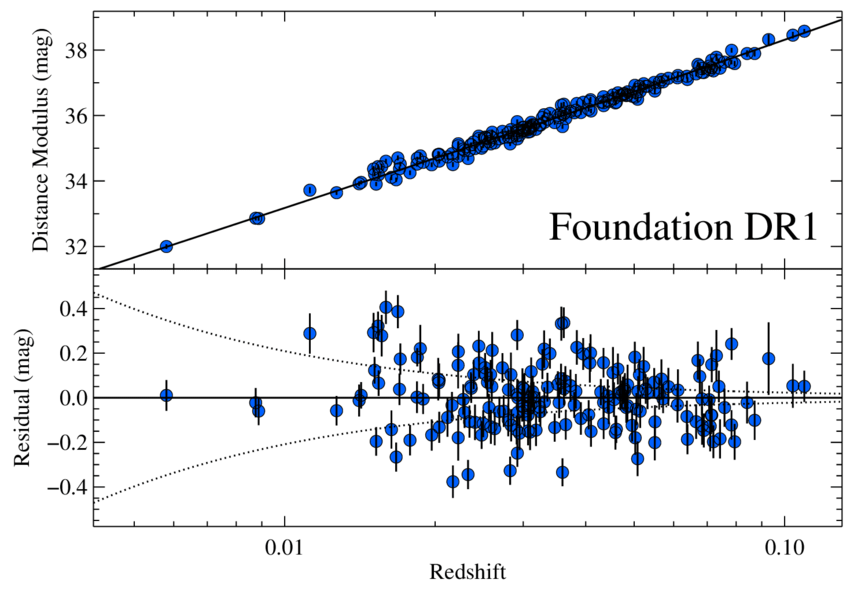
\includegraphics[width=0.8\textwidth]{figs/hubble-resid.png}
    \caption{A Hubble diagram (top) made with SNe Ia. The Hubble residual is plotted in the lower panel. The curved dotted lines in the lower panel mark error due to peculiar velocity. Figure from \cite{Foley2017}.}
    \label{fig:hresid}
\end{figure}

There are some nuances---for one, not all of the components of a galaxy's velocity are moving away in accordance with the Universe's expansion. This is called the \textit{Hubble flow}---if an object is \textit{only} moving due to expansion, then it's in the Hubble flow. Any velocity deviation from the Hubble flow is called \textit{peculiar velocity}. For example, if a galaxy is under gravitational influence from another galaxy, the components of its motion due to that interaction is part of its peculiar velocity. However, this is hard to quantify, so it's usually assumed that peculiar velocity is around 300 km/s. You'll notice that in plots that show peculiar velocity error, like in the lower panel of Figure \ref{fig:hresid}, the error due to peculiar velocity gets smaller as an object is farther away. 

Peculiar velocity error is calculated as:
\begin{equation}
    \sigma_{v_{pec}} = \Big( \frac{5}{\ln 10} \Big) \Big( \frac{v_{pec}}{cz} \Big)
\end{equation}
So, it's a function of $z$! This makes sense---the farther away something is, the faster it's moving in the Hubble flow, so the peculiar velocity is a relatively small portion of its net velocity vector. 

While you'll plot those curved dotted lines as peculiar velocity error alone, you should add the error due to peculiar velocity in quadrature (i.e. sum the errors like $\sigma = \sqrt{a^{2} + b^{2}}$) to the error bars on your data.

\subsection{Important papers for supernova cosmology}

\textit{The Use of Supernovae Light Curves for Testing the Expansion Hypothesis and Other Cosmological Relations}, B. Rust's PhD thesis, 1974 \cite{Rust1974}. The author shows that SNe Ia can be used to test the expanding Universe hypothesis.\\

\noindent\textit{Light curves, color curves, and expansion velocity of type I supernovae as functions of the rate of brightness decline}, I. Pskovskii 1977 \cite{Pskovskii1977}. This is the first paper to quantify the rate of brightness decline. It was quantified as $\beta$, which paved the way for $\Delta m_{15}$ much later \cite{Phillips1993}. \\

\noindent\textit{The Absolute Magnitudes of Type Ia Supernovae}, M. Phillips 1993 \cite{Phillips1993}. This paper shows that the absolute magnitudes of SNe Ia are correlated with the decline rate of the $B-$band light curve. This paper is why the luminosity-decline relation is sometimes called the ``Phillips relation''. This paper quantifies the brightness decline rate as $\Delta m_{15}$---the change in magnitude from the date of maximum brightness to 15 days later.\\

\noindent\textit{Dr. Paulina Lira's Masters thesis}, 1995. This thesis notes a linear region in the color curve (color vs. time) of SNe Ia. This is suggested as a method to correct reddening. \\

\noindent\textit{The Reddening-Free Decline Rate Versus Luminosity Relationship for Type IA Supernovae}, M. Phillips et al. 1999. \cite{Phillips1999}. This paper elaborates on Phillips 1993 \cite{Phillips1993}. It modifies the previously-described luminosity-decline relation by correcting for host galaxy extinction using the relation in Lira 1995.\\

\noindent\textit{Observational Evidence from Supernovae for an Accelerating Universe and a Cosmological Constant}, Riess et al. 1998 \cite{Riess1998}. This is the paper that won the Nobel Prize in 2011, awarded to Adam Riess, Saul Perlmutter, and Brian Schmidt. The authors used High-$z$ Supernova Search Team data combined with some nearby SNe to show that the distances of the high $z$ SNe were larger than expected, implying that the Universe is expanding at an accelerating rate. The Supernova Cosmology Project group found the same results at around the same time.\\
\section{Photometry}
\section{Spectra}
\subsection{Correcting to the rest frame}
\label{sec:spec_restframe}
Correcting the observed wavelength for the relativistic Doppler effect is done by: 
\begin{equation}
    \lambda_{rest \,\, frame} = \frac{\lambda_{observed}}{1+z_{helio}}.
\end{equation}

Correcting the observed flux is more complicated and I've redacted this section for now. If you need to correct flux to the rest frame, see the next section and normalize to a chosen $z$. 

\subsection{Normalizing to a particular $z$}
Sometimes, you want your spectrum flux as if it were at some redshift $z_{ref}$ that you've chosen. Do not use the rest frame spectrum for this calculation. First thing's first, you need the luminosity distance to your object.

\begin{equation}
    D_{L} = (1+z_{helio})D_{M},
\end{equation}

where $z_{helio}$ is the heliocentric ($\sim$observed) redshift for your object, and $D_{M}$ is the comoving transverse distance. In Python, you can use \texttt{astropy.cosmology}'s function \texttt{comoving\_transverse\_distance}, which takes $z_{CMB}$ as its input (so you'll also need your object's RA and dec), to calculate $D_{M}$. If we assume an FLRW universe, then our cosmological scale factor is $a(t) = 1/(1+z)$. Then,
\begin{equation}
    \frac{a(t_{ref})}{a(t_{actual})} = \Big( \frac{1 + z_{helio}}{1+z_{ref}} \Big) \Big( \frac{D_{L, actual}}{D_{L, ref}} \Big)^{2}
\end{equation}

Finally, convert your flux by using this value:
\begin{equation}
    F_{ref} = F_{actual}\Big( \frac{1 + z_{helio}}{1+z_{ref}} \Big) \Big( \frac{D_{L, actual}}{D_{L, ref}} \Big)^{2} = F_{actual} \Big(\frac{a(t_{ref})}{a(t_{actual})} \Big)
\end{equation}

Using Equation~\ref{eqn:errorprop}, the error is:
\begin{equation}
    \sigma_{F_{ref}} = \sigma_{F_{actual}}\frac{\partial F_{ref}}{\partial F_{actual}} = \sigma_{F_{actual}}\Big( \frac{1 + z_{helio}}{1+z_{ref}} \Big) \Big( \frac{D_{L, actual}}{D_{L, ref}} \Big)^{2}
\end{equation}

\subsection{Absorption lines}
\subsubsection{Pseudo-equivalent width}
Pseudo-equivalent width (pEW) is a measure of the strength of an absorption line. It combines the depth and the width of the line into one measurement by integrating over the feature. There's a really good run-down of pEW in \cite{Galbany2015}. So, we're going to borrow from them. Figure~\ref{fig:pew} shows an absorption feature. You start with one like the one on the left (red). We want to measure the strength of the absorption feature, but the problem with SNe is that there are so many absorption and emission lines and there's doppler shift everywhere, so we don't really know where the continuum is. \textit{But}, we need a way to fairly compare absorption features between different SNe, which means removing the continuum. So, we make a ``pseudo-continuum'' to approximate a small region of the actual continuum. Lines are nice, so all you do to make the pseudo-continuum is draw a line across the top of the absorption feature. We remove the ``continuum'' by normalizing the absorption feature to the pseudo-continuum. You only do this for the one feature---for each absorption feature, you need a new pseudo-continuum. After you've normalized to the pseudo-continuum, you end up with the \textit{right} panel of Figure~\ref{fig:pew} (green). Now, you can measure the area and fairly compare line strengths between SNe. 

\begin{figure}[h!]
    \centering
    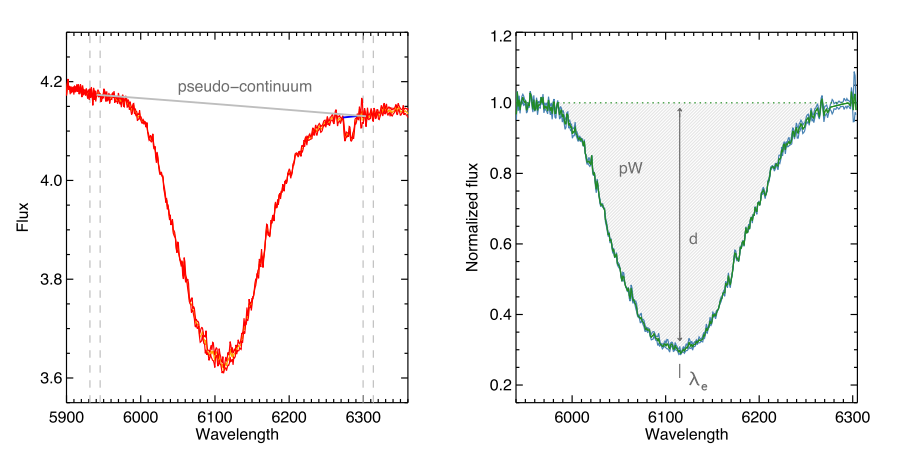
\includegraphics[width=0.9\textwidth]{figs/Screenshot from 2022-07-12 16-05-37.png}
    \caption{\textit{Left}: Un-normalized absorption feature. \textit{Right}: The same absorption feature normalized to the pseudo-continuum marked on the \textit{left}. $d$ is the feature depth and $\lambda_{e}$ is the center wavelength. The shaded area is the pEW (pW in the figure). Figure from \cite{Galbany2015}.}
    \label{fig:pew}
\end{figure}

That's great and all, but how do we actually do all this in practice? There are a lot of ways. Let's break it down into steps and talk about 'em. This is \textit{not} an exhaustive list, nor is it the only way to do this---these are merely suggestions. Let your imagination run free, spectral padawan.

\begin{enumerate}
    \item \textbf{Finding the pseudo-continuum:} The challenging part of this step is avoiding noise. We don't want an unrealistic pseudo-continuum because we picked a point where there's a statistical spike or dip in the measurement. You can smooth the data with a moving average, or use the Savitzky-Golay filter from \texttt{scipy.signal.savgol\_filter()}. Discussing the differences between these two is outside the scope of this manual, but you should always understand the techniques you're using! 
    \item \textbf{Normalizing to the pseudo-continuum:} Take your smoothed flux and divide by the line you drew. Here's some Python-inspired pseudo-code to help you out:
    \begin{minted}[
    bgcolor=lightgray,
    frame=leftline,
    framesep=-3mm]
    {python}
    continuum = scipy.interpolate.interp1d(flux[start_point],
        flux[end_point])
    normalized_flux = flux[start_point:end_point]
        /continuum(wavelength[start_point:end_point])
    \end{minted}
    
    \item \textbf{Integrating over the absorption feature:} You can do this via summation directly over the normalized data or by fitting a Gaussian and integrating that. 
\end{enumerate}

Now... we weren't going to have this entire discussion without talking about error on pEW, of course. The error for this kind of ``guesstimation'' thing is hard to quantify precisely, so I recommend a bootstrapping method like the one in \cite{Galbany2015}. Instead of choosing fixed endpoints for your pseudo-continuum, draw randomly from some small region around your chosen endpoints $N$ times to get $N$ sets of different, but all reasonable, endpoints. Now, calculate the pEW as discussed above for each set of endpoints. Then, your final pEW measurement is the mean of all $N$ measurements, with the standard deviation of all $N$ measurements as your error on pEW. 

\subsubsection{Ejecta velocity}
\label{sec:ejectavelocity}

\subsection{Synthetic photometry}

If you're here, you're wondering how to make photometry from some spectra. In short, this is obtained by integrating under the spectrum in the region covered by a given filter. 

The area under the spectrum, $F$, in a given filter $X$, is calculated by
\begin{equation}
    F_{X} = \frac{1}{hc}\int_{\lambda_{1}}^{\lambda_{2}} \lambda f(\lambda) R_{X}(\lambda) d\lambda,
\label{eqn:synthint}
\end{equation}

where $f(\lambda)$ is your spectrum, and $R_{X}(\lambda)$ is your filter. The $\lambda$ and $1/hc$ terms are in there if we're using photon-counting detectors, and using an input spectrum that's in energy units. If you're using an energy-counting detector, you would drop this, i.e., your integrand is $f(\lambda) R_{X}(\lambda) d\lambda$.

However, we can't often use the continuous version of this function with our data. So, we discretize it:

\begin{equation}
    F_{X} = \frac{1}{hc}\sum_{i=\lambda_{1}}^{\lambda_{2}} \lambda_{i} f(\lambda_{i}) R_{X}(\lambda_{i})(\lambda_{i} - \lambda_{i-1}),
\label{eqn:synth_discrete}
\end{equation}

where $f(\lambda_{i})$ is the energy flux at a particular wavelength $\lambda_{i}$, and $R_{X}(\lambda_{i})$ is the response function for the filter at wavelength $\lambda_{i}$. We're using a discretized version of an integral, so $(\lambda_{i} - \lambda_{i-1})$ is the same as $d\lambda$. From now on, this chapter will be written as if we are using Equation \ref{eqn:synth_discrete}.

Then, for a photon-counting detector with an input spectrum in units of energy, the variance of $F$ (using Equation \ref{eqn:errorprop}) is:

\begin{equation}
\label{eqn:varphot}
    \sigma_{F}^{2} = \frac{1}{(hc)^{2}}\sum_{i=\lambda_{1}}^{\lambda_{2}} \lambda_{i}^{2}\sigma_{f(\lambda_{i})}^{2} R_{X}(\lambda_{i})^{2}(\lambda_{i} - \lambda_{i-1})^{2} 
\end{equation}

For an energy-counting detector with an input spectrum in units of energy, the variance of $F$ is:
\begin{equation}
\label{eqn:varenergy}
    \sigma_{F}^{2} = \sum_{i=\lambda_{1}}^{\lambda_{2}} \sigma_{f(\lambda_{i})}^{2} R_{X}(\lambda_{i})^{2}(\lambda_{i} - \lambda_{i-1})^{2} 
\end{equation}

Individual magnitudes are calculated by
\begin{equation}
    m = -2.5\log_{10}\Big(\frac{F}{F_{ref}}\Big) = -2.5\log_{10}(F) + 2.5\log_{10}(F_{ref}) = -2.5\log_{10}(F) - m_{ref}.
\end{equation}
\textit{Wait---what are $F_{ref}$ and $m_{ref}$}? Good question. Because magnitudes are inherently relative quantities, we need to use some reference object to convert flux into magnitudes. You can get reference objects from \href{https://www.stsci.edu/hst/instrumentation/reference-data-for-calibration-and-tools/astronomical-catalogs/calspec}{CALSPEC}. Photometric systems are, unfortunately, out of the scope of this manual at this time. Let's say we're using the Vega system, with the star Vega (Alpha Lyrae) from now on. 

This means we need to use Equation \ref{eqn:synth_discrete} on our reference object, Vega to calculate $F_{ref}$. You'll use the \textit{same} response function as you use for your supernova spectrum. This means that $m_{ref}$ is the... reference magnitude? What does THAT mean? If magnitudes are inherently relative quantities, do we then compare our reference object to something \textit{else}? A valid concern, but no! This is called a \textit{zero point}. For the Vega system, astronomers have defined the magnitude of the star Vega such that the $m_{Vega}$ = 0 in all bands. So, if you're using the Vega system, $m_{ref}$ is probably just 0 (unless some literature tells you otherwise, which is possible, so make sure you're familiar with the photometric system and filters you're using).

So anyway, the variance of $m$ (for an energy-counting detector) is:
\begin{equation}
    \sigma_{m}^{2} = \frac{\partial m}{\partial f}^{2} \sigma_{f}^{2} = \frac{\partial m}{\partial F}^{2} \Big( \sum_{i=\lambda_{1}}^{\lambda_{2}} \frac{\partial F}{\partial f(\lambda_{i})} \sigma_{f(\lambda_{i})}\Big)^{2} = \Big( \frac{-2.5}{F\ln10} \Big)^{2} \sum_{i=\lambda_{1}}^{\lambda_{2}}\sigma_{f(\lambda_{i})}^{2} R_{X}(\lambda_{i})^{2}(\lambda_{i}-\lambda_{i-1})^{2}
    \label{eqn:m_err}
\end{equation}

Note that the summation term on the right-hand side of the equation is the same as $\sigma_{F}^{2}$. You need to be careful about flux variance here, though: Equations~\ref{eqn:synth_discrete},   \ref{eqn:varphot}, and \ref{eqn:varenergy} are true, but when you are calculating magnitudes, keep in mind that you're calculating this based off a relative flux. So, your flux variance should also be relative. In other words, it should be the variance of $F/F_{ref}$. Using Equation~\ref{eqn:errorprop} and treating $F_{ref}$ as a constant, we get

\begin{equation}
    \sigma^{2}_{F/F_{ref}} = \frac{1}{F_{ref}^{2}}\sum_{i=\lambda_{1}}^{\lambda_{2}} \lambda_{i}\sigma_{f(\lambda_{i})}^{2} R_{X}(\lambda_{i})^{2}(\lambda_{i} - \lambda_{i-1})^{2} 
\end{equation}

(or the equivalent energy-counting version of this). Note that we do not account for error on $F_{ref}$, here. That's why we just use $\sigma_{f(\lambda_{i})}$, which is the error of your data spectrum. \\

If you're looking for \textit{colors}, I've got your back there, too. For arbitrary color $X-Y$,
\begin{equation}
    m_{X} - m_{Y} = -2.5\log \Big( \frac{F_{X}}{F_{ref,X}} \Big) + 2.5\log \Big( \frac{F_{Y}}{F_{ref,Y}} \Big).
\end{equation}
We can propagate the error here, too. If you want, you can assume $X$ and $Y$ are independent, and do $\sigma_{X-Y} = \sqrt{\sigma_{X}^{2} + \sigma_{Y}^{2}}$. However, we can be more rigorous and not assume independence. We're going to use $\sigma^{2} = \mathbf{JCJ^{T}}$---the explanation of this formula is beyond the scope of this manual. $\mathbf{J}$ is the Jacobian of your spectrum (remember, your spectrum is a function!), and $\mathbf{C}$ is its covariance matrix. The following method will work \textit{if you have an error for the flux in your data spectrum}.

For ease of calculations, we will treat $m_{X}-m_{Y}$ as a function of $f(\lambda_{i})$ (our supernova spectrum, in discrete wavelength chunks). Then, for arbitrary color $X-Y$, the Jacobian is:
\begin{equation}
\label{eqn:jac2}
\mathbf{J}_{X-Y} = 
\begin{bmatrix}
    
        \frac{\partial m_{X-Y}}{\partial f(\lambda_{0})} & \frac{\partial m_{X-Y}}{\partial f (\lambda_{1})} & \dots & \frac{\partial m_{X-Y}}{\partial f(\lambda_{N})} \\
    
\end{bmatrix}
\end{equation}

\parindent = 0 mm

where $N$ is the last measured wavelength in the spectrum. The $i$th entry is: 
\begin{equation}
    \frac{\partial m_{X-Y}}{\partial f(\lambda_{i})} = -\frac{1.09}{F_{X}} R_{X}(\lambda_{i})(\lambda_{i}-\lambda_{i-1}) + \frac{1.09}{F_{Y}}R_{Y}(\lambda_{i})(\lambda_{i}-\lambda_{i-1})
\end{equation}

Then, the covariance matrix is diagonal, and each entry is the spectrum error provided in the data:
\begin{equation}\mathbf{C_{X-Y}} = 
    \begin{bmatrix}
        \sigma_{f(\lambda_{0})}^{2} &  & & \\
         & \sigma_{f(\lambda_{1})}^{2}&  & \\
         &  & \ddots &  \\
        & & & & \sigma_{f(\lambda_{N})}^{2}\\
    \end{bmatrix}.
    \label{eqn:cov}
\end{equation}
Now, we use $\sigma^{2} = \mathbf{JCJ^{T}}$, and boom, we have color error without assuming independence for the filters. 

\subsection{Things to watch out for}
\subsubsection{Response function units}
Your response function will likely be normalized, but may be given in either normalized flux units or normalized photon counts. You need to know which units you have. If you need the other, don't fret---you can convert it to the other unit system. Let's say you have a response function in normalized photon units, but your spectrum is in energy flux units (ergs/cm$^{2}$/s/$\mathrm{\AA}$). It's best to convert the spectrum to photons. For each $i$th wavelength, you do:

\begin{equation}
    f_{\gamma}(\lambda_{i}) = \frac{\lambda_{i}}{hc}f_{E}(\lambda_{i}),
\end{equation}
where $h \approx 6.626 \times 10^{-27}$ ergs $\cdot$ s and $c \approx 3\times 10^{18}$ is the speed of light in $\mathrm{\AA}$/s. 

Why convert the spectrum instead of the response function? Well, CCDs count photons, so it's ideal to do as much as possible in these units. \\

Don't forget to convert your errors, as well. Using Equation~\ref{eqn:errorprop},

\begin{equation}
    \sigma_{f_{\gamma}(\lambda_{i})} = \frac{\lambda_{i}}{hc}\sigma_{f_{E}(\lambda_{i})}.
\end{equation}

\subsubsection{Help! My results are unreasonable!}

Did you check all of the following:
\begin{itemize}
    \item Did you convert both your standard spectrum \textit{and} your data spectrum from ergs to photons (or vice versa)?
    \item When you converted between ergs and photons, did you use the correct units for the constants? Remember, for ergs/cm$^{2}$/s/$\mathrm{\AA}$, use $h \approx 6.626 \times 10^{-27}$ ergs $\cdot$ s and $c \approx 3\times 10^{18}$ $\mathrm{\AA}$/s. 
    \item When you converted between ergs and photons, did you multiply by the conversion factor when you should have divided (or vice versa)? 
    \item Does the wavelength range of your filter fall completely inside the wavelength range of your spectrum? 
    \item Did you convert units when maybe you shouldn't have because you already did it? 
\end{itemize}

\section{Classifying spectra}
You can use \href{https://people.lam.fr/blondin.stephane/software/snid/}{SNID} or the in-browser option \href{https://gelato.tng.iac.es/gelato/}{GELATO}. Tutorials forthcoming. 
\section{Software and Models}
\label{sec:software}
\subsection{SALT}
\subsubsection{What is SALT?}


\subsubsection{Models}
\textit{SALT: a spectral adaptive light curve template for type Ia supernovae}, J. Guy et al. 2005 \cite{salt}. This is the first SALT model. The model is trained on 34 SNe with $z < 0.1$ in $UBVRI$ filters. \\

\textit{SALT2: using distant supernovae to improve the use of type Ia supernovae as distance indicators}, J. Guy et al. 2007 \cite{salt2}. SALT is retrained on data with $z \leq 1$. \\

\textit{Improved cosmological constraints from a joint analysis of the SDSS-II and SNLS supernova samples}, M. Betoule et al. 2014 \cite{salt2.4}. SALT2 is retrained on the data from \cite{salt2}, with the addition of SDSS-II data, for $z < 0.25$. SALT2.4 is born. \\

\textit{SALT3: An Improved Type Ia Supernova Model for Measuring Cosmic Distances}, W. D. Kenworthy et al. 2021 \cite{salt3}. SALT2.4 gets a facelift and becomes more open-sourcey. \\

\textit{SALT3-NIR: Taking the Open-source Type Ia Supernova Model to Longer Wavelengths for Next-generation Cosmological Measurements}, J. D. R. Pierel et al. 2022 \cite{salt3nir}. SALT3 gets upgraded to include NIR wavelengths. 

\subsubsection{How do I use SALT models?}
SALT3 is in several places. You can use these models through:
\begin{itemize}
    \item \href{https://sncosmo.readthedocs.io/en/stable/}{\texttt{sncosmo}} (You can use \texttt{SNANA} models in \texttt{sncosmo}, as well.)
    \item \href{https://github.com/RickKessler/SNANA}{\texttt{SNANA}} (SALT2 only)
\end{itemize}

I haven't used \texttt{SNANA}, so I can't help you with that. However, Section \ref{sec:sncosmo} contains tips on using \texttt{sncosmo}. 

\subsection{sncosmo}
\label{sec:sncosmo}
\href{https://github.com/sncosmo/sncosmo}{\texttt{sncosmo}} is pretty cool. It has a whole bunch of contributors. It's a Python package, useful for middle steps of supernova cosmology (e.g., fitting models). You can fit a \href{https://sncosmo.readthedocs.io/en/stable/source-list.html}{lot of stuff} with it, actually. \texttt{sncosmo} provides fit parameters for your data. You can use either spectroscopic or photometric data.

\subsubsection{Fitting a light curve with photometry}
You \textit{must} input flux units into \texttt{sncosmo} in order for it to work. Trust me, I've tried using it with magnitudes because I was in denial that I would have to do a unit conversion (boo hoo). These should be \textit{physical flux of your object, not flux of an object in a particular magnitude system} (see \ref{sec:magtoflux}).\\

First, your data needs to be in an \texttt{astropy} table with columns\\
\texttt{[`date',`flux',`fluxerr',`band',`zp',`zpsys']}. 

\subsubsection{Converting SALT parameter output to magnitude error along your entire light curve}

\texttt{sncosmo} contains a function for converting your model fit to a light curve with covariance: \texttt{Model.bandfluxcov()}. You'd use it like this:

\begin{minted}[
    bgcolor=lightgray,
    frame=leftline,
    framesep=-3mm]
    {python}

    import sncosmo 
    import numpy as np
    from astropy import Table
    import pandas as pd

    # Read in your data:
    csv = pd.read_csv('SN2014J.csv')
    # Define band and magnitude system:
    band = 'B'
    phase = np.arange(-10,30,0.1)
    vega = sncosmo.get_magsystem('vega')

    # Turn your pandas table into an astropy table
    # so sncosmo can use it, and fit the model. 
    data = Table.from_pandas(csv)
    model = sncosmo.Model(source='salt3')
    result, fitted_model = sncosmo.fit_lc(data, model, 
        ['t0', 'x0', 'x1', 'c'])

    flux_lc, cov = fitted_model.bandfluxcov(band, phase)      

\end{minted}

where \texttt{flux\_lc} is an array of the flux through your \texttt{band} at all phases in \texttt{phase}. Because I did \textit{not} provide the zero point or zero point system as an argument (\texttt{`zp'} and \texttt{`zpsys'}, respectively), this is the physical flux of the object through the bandpass, \texttt{band} in photons/s/cm$^{2}$. \texttt{cov} is an $n \times n$ symmetric matrix, where $n$ is the length of your \texttt{phase} array. Its entries contain the covariance between band fluxes at different phases. \\

However, \textit{you need to provide \texttt{zp} and \texttt{zpsys} to \texttt{Model.bandfluxcov()} if you are converting to magnitudes, because magnitudes are a relative unit system}. You could also use the ``hidden'' function \texttt{Model.\_bandflux\_rcov()} to calculate the covariances. This calculates the \textit{relative} covariance---i.e., covariances that are \textit{fractions} of the flux. So, if you do this, you need to remember to multiply your covariance matrix by the flux. You can take the diagonal entries of the covariance matrix output from \texttt{Model.\_bandflux\_rcov()}, invoking the assumption that all phases are independent measurements, and convert these to magnitudes using Equation \ref{eqn:errorprop} (or, to skip doing derivatives yourself, Equation \ref{eqn:flux-to-mag-err}). Like so: \\

\begin{minted}[
    bgcolor=lightgray,
    frame=leftline,
    framesep=-3mm]
    {python}

    import sncosmo 
    import numpy as np
    from astropy import Table
    import pandas as pd

    # Read in your data:
    csv = pd.read_csv('SN2014J.csv')
    # Define band and magnitude system:
    band = 'B'
    phase = np.arange(-10,30,0.1)
    vega = sncosmo.get_magsystem('vega')
    # See the section on zeropoint trouble
    # in sncosmo for an explanation of this line:
    zeropoint = csv['mag'] + 
    2.5*np.log10*(vega.band_mag_to_flux(csv['mag'], band)

    # Turn your pandas table into an astropy table
    # so sncosmo can use it, and fit the model. 
    data = Table.from_pandas(csv)
    model = sncosmo.Model(source='salt3')
    result, fitted_model = sncosmo.fit_lc(data, model, 
        ['t0', 'x0', 'x1', 'c'])

    flux_lc, cov = fitted_model.bandfluxcov(band, phase, 
        zp=zeropoint, zpsys=vega) 

    flux_err = np.sqrt(cov.diagonal()) # Multiply flux_err by flux_lc
                                       # if you use _bandflux_rcov().
    mag_err = np.sqrt(((2.5/np.log(10))**2)*(1/(flux_lc**2)) 
        *flux_err**2) 
    

\end{minted}

\subsubsection{\texttt{helio\_to\_cmb()}}
\label{sec:heliotocmb}
The below code is handy for converting your heliocentric redshift to CMB redshift. Honestly, I can't find its location in the sncosmo github right now, so I've copied and pasted it below: 

\begin{minted}[
    bgcolor=lightgray,
    frame=leftline,
    framesep=-3mm]
    {python}
    
    import math
    import numpy as np
    from astropy.coordinates import SkyCoord
    
    # From sncosmo:
    def radec_to_xyz(ra, dec):
        # SUPERNOVA BOOTCAMP MANUAL AUTHOR ADDITION: 
        # Modified to add the try/except statement
        try:
            x = math.cos(np.deg2rad(dec)) 
                * math.cos(np.deg2rad(ra))
            y = math.cos(np.deg2rad(dec)) 
                * math.sin(np.deg2rad(ra))
            z = math.sin(np.deg2rad(dec))
        except:
            coord = SkyCoord('%s %s' % (ra, dec), 
                unit=(u.hourangle,u.deg))
            x = math.cos(np.deg2rad(coord.dec.degree)) 
                * math.cos(np.deg2rad(coord.ra.degree))
            y = math.cos(np.deg2rad(coord.dec.degree)) 
                * math.sin(np.deg2rad(coord.ra.degree))
            z = math.sin(np.deg2rad(coord.dec.degree))
    
        return np.array([x, y, z], dtype=np.float64)
    
    def cmb_dz(ra, dec):
        # See http://arxiv.org/pdf/astro-ph/9609034
        CMBcoordsRA = 167.98750000 # J2000 
        CMBcoordsDEC = -7.22000000
    
        # J2000 coords from NED\n",
        CMB_DZ = 371000. / 299792458.
        CMB_RA = 168.01190437
        CMB_DEC = -6.98296811
        CMB_XYZ = radec_to_xyz(CMB_RA, CMB_DEC)
        coords_xyz = radec_to_xyz(ra, dec)
        dz = CMB_DZ * np.dot(CMB_XYZ, coords_xyz)
    
        return dz

    def helio_to_cmb(z, ra, dec):
        # Convert from heliocentric redshift to CMB-frame redshift.
        "    Parameters\n",
        "    ----------\n",
        "    z : float\n",
        "        Heliocentric redshift.\n",
        "    ra, dec: float\n",
        "        RA and Declination in degrees (J2000).\n",
        "    \"\"\"\n",
    
        dz = -cmb_dz(ra, dec)
        one_plus_z_pec = math.sqrt((1. + dz) / (1. - dz))
        one_plus_z_CMB = (1. + z) / one_plus_z_pec
    
        return one_plus_z_CMB - 1.
\end{minted}

\subsubsection{Help! I'm having zero point trouble.}
\label{sec:zeropointsncosmo}
First, make sure you're inputting \textit{physical flux units}, not the flux of your object in a magnitude system. If you converted from magnitudes to flux, this is likely to be the issue (see section \ref{sec:magtoflux}). So, what you need to do is take your reference spectrum back out of your magnitude.\\

Now, if you've done this, you can't forget to also convert your magnitude errors back to flux errors. It's the same equation as the error equation in \ref{sec:magtoflux}. No funny business with the conversion back to physical units because that's just a constant offset, so the derivative from Equation \ref{eqn:errorprop} takes it out. \\

Here's some Python code to help you out with this fix: 
\begin{minted}[
    bgcolor=lightgray,
    frame=leftline,
    framesep=-3mm]
    {python}
    
    import sncosmo 
    import numpy as np
    from astropy import Table
    import pandas as pd

    # Read in your data:
    csv = pd.read_csv('SN2014J.csv')
    # Define band and magnitude system:
    band = 'B'
    vega = sncosmo.get_magsystem('vega')

    # This is the line where you calculate the offset to 
    # remove the Vega spectrum:
    zeropoint = data['mag'] + 
        2.5*np.log10*(vega.band_mag_to_flux(data['mag'], band)

    # Throw that offset into your table:
    data['zp'] = pd.Series([zeropoint 
        for x in range(len(data.index))])

    # Calculate your flux error (absolute value because it's
    # squared and then square-rooted):
    data['fluxerr'] = abs((data['magerr']*np.log(10)/2.5)*
        (vega.band_mag_to_flux(data['mag'], band))

    # Turn your pandas table into an astropy table
    # so sncosmo can use it, and fit the model. 
    data = Table.from_pandas(csv)
    model = sncosmo.Model(source='salt3')
    result, fitted_model = sncosmo.fit_lc(data, model, 
        ['t0', 'x0', 'x1', 'c'])
    
\end{minted}

\subsection{SNooPy}
\href{https://csp.obs.carnegiescience.edu/data/snpy}{SNooPy} \cite{snoopy1,snoopy2}, written in Python by Chris Burns for the Carnegie Supernova Project, has a lot of handy functions. Broadly, it is a Python package that fits light curves, but it's broken up into a lot of separate functions, which can be very useful. You can run SALT2 and MLCS2k2 models via SNooPy, as well. 


Below, I'll list some of my favorite functions that are not-so-discussed in the \href{https://csp.obs.carnegiescience.edu/data/snpy/documentation}{documentation}. 

\subsubsection{\texttt{get\_dust\_RADEC()} and \texttt{get\_dust\_sigma\_RADEC()}}
\label{sec:snpydustfuncs}

\par
\texttt{get\_dust\_RADEC()} and \texttt{get\_dust\_sigma\_RADEC()} query \href{https://irsa.ipac.caltech.edu/frontpage/}{IRSA} using a given RA and dec to get the Milky Way $E(B-V)$ and error in $E(B-V)$, respectively. These are located in \texttt{snpy.utils.IRSA\_dust\_getval}. They accept arguments for RA and dec, with the default dust map from \cite{sf11dust}. They return two things: the result and a flag. The flag indicates that the function worked. You can throw this out. \\

\noindent\textbf{Usage example:}
\begin{minted}[
    bgcolor=lightgray,
    frame=leftline,
    framesep=-3mm]
    {python}
    from snpy.utils.IRSA_dust_getval import get_dust_RADEC, 
        get_dust_sigma_RADEC

    '''
    SN 1987A coordinates from 
    http://simbad.u-strasbg.fr/simbad/sim-id?Ident=SN+1987A.
    Note: At the time of writing this, the get_dust_RADEC()
    function works, but get_dust_sigma_RADEC() is failing.
    Otherwise, this code works as-is.
    '''

    ra, dec = 279.703427, -31.937066
    mwreddening,_ = get_dust_RADEC(ra, dec, calibration='SF11')
    e_mwreddening,_ = get_dust_sigma_RADEC(ra, dec, 
        calibration='SF11')
    mwreddening = mwreddening[0]
    e_mwreddening = e_mwreddening[0]

    print(f'The Milky Way reddening for SN 1987A is {mwreddening}
        +/- {e_mwreddening}.')

\end{minted}

\subsection{mpfit}
\label{sec:mpfit}
\texttt{mpfit} is a very flexible Levenberg-Marquardt $\chi^{2}$ minimization code. It can take error in both the $x$ and $y$ axes into account. It's useful to be familiar with! The Python code is located \href{https://github.com/segasai/astrolibpy/blob/master/mpfit/mpfit.py}{here}. What I think you should do with this is download this *.py file, and make it so it's importable. Then, write some functions that make it easier to use:

\begin{minted}[
    bgcolor=lightgray,
    frame=leftline,
    framesep=-3mm]
    {python}
    import os, sys
    import numpy as np

    # The next two lines assume that you are making this file
    # in the same directory as the ``mpfit'' directory. i.e.,
    # /home/this_file.py
    # and
    # /home/mpfit/mpfit/mpfit.py
    dirname = os.path.dirname(os.path.abspath(__file__))
    sys.path.append(os.path.join(dirname,'mpfit'))
    
    from mpfit import mpfit
    
    def Flin(x,p):
        """
        Set up linear function for mpfit to use. 
        You can use any kind of function you want, though.
        The line is just an example.
        DO NOT call this.
        """
        y =  p[0] + p[1]*x 
        return y
    
    def myfunctlin(p, fjac=None, x=None, y=None, xerr=None, 
        yerr=None):
        """
        Set up chisq to minimize for mpfit. This will accept any
        combination of xerr and yerr (i.e., you do not need either, 
        or both).
        DO NOT call this. 
        """
        # Parameter values are passed in "p".
        # If fjac==None then partial derivatives should not be
        # computed.  It will always be None if MPFIT is called 
        # with the default flag.
        model = Flin(x, p)
        # Positive status value means MPFIT should continue, 
        # negative means stop the calculation.
        status = 0

        # If you don't use the line function, you need 
        # to change this and write your own chi^2 here.
        if xerr is not None and yerr is not None:
            return [status, np.sqrt((y-model)**2/(yerr**2 + 
                (p[1]**2)*xerr**2))]
        elif xerr is None and yerr is not None:
            return [status, np.sqrt((y-model)**2/(yerr**2))]
        elif xerr is not None and yerr is not None:
            return [status, np.sqrt((y-model)**2/((p[1]**2)*xerr**2))]
        elif xerr is None and yerr is None:
            return [status, y-model]
    
    def linfit(x,y,ex=None, ey=None, initial_guess=[0,1]):
        """
        Do the linear fit. USE THIS FUNCTION DIRECTLY IN YOUR CODE. 
        i.e., you'd write something like:
        from this_file import linfit
        """
        # p0 are the initial conditions
        p0=np.array(initial_guess,dtype='float64') 
        if ex is not None and ey is not None:
            fa = {'x':x, 'y':y, 'xerr': ex, 'yerr': ey}
        elif ex is None and ey is not None:
            fa = {'x':x, 'y':y, 'yerr': ey}
        elif ex is not None and ey is None:
            fa = {'x':x, 'y':y, 'xerr': ex}
        elif ex is None and ey is None:
            fa = {'x':x, 'y':y}
        m = mpfit(myfunctlin, p0, functkw=fa)
        return m.params, m.covar
\end{minted}

\section{Packaging your code in Python}

This is possibly the most useful thing that I ever learned to do in graduate school. First of all, I'd like to give props to \href{https://semaphorep.github.io/codeastro/}{Code/Astro} for being an incredible workshop where I learned this. This tutorial will be the barest, most barebones way to package your stuff. This will not cover things like unit tests, licenses, or documents.\\

Let's say we have a file, \texttt{calculate\_magnitudes.py}. It looks like this:

\begin{minted}[
    bgcolor=lightgray,
    frame=leftline,
    framesep=-3mm]
    {python}
    import numpy as np

    def calc_mag(f):
        return -2.5*np.log10(f)
\end{minted}

and we want to be able to import it into a different file because it's an enormous collection of functions and you don't want to copy and paste that monster (just use your imagination, okay?). Let's name our package \texttt{magpy}. You will make a folder with the following structure and contents:

\begin{minted}[
    bgcolor=lightgray,
    frame=leftline,
    framesep=-3mm]
    {python}
    > magpy
        > calculate_mag
            calculate_magnitudes.py
            __init__.py
        README.md
        requirements.txt
        setup.py
\end{minted}

Let's talk about what each of these are, and what goes in each of them. \\

\texttt{> magpy} --- This folder contains everything. It is the highest-level directory in the package.\\

\texttt{> calculate\_mag} --- This folder contains your code. It may also have accompanying data files. \\

\texttt{calculate\_magnitudes.py} --- This is your code. Your functions and tools you want to use exist in here. \\

\texttt{\_\_init\_\_.py} --- This file is run when you first import the package. If you don't want to write a long string of stuff like \\\texttt{from magpy.calculate\_mag.calculate\_magnitudes import calc\_mag}, write the following in this file:

\begin{minted}[
    bgcolor=lightgray,
    frame=leftline,
    framesep=-3mm]
    {python}
    from .calculate_magnitudes import *
\end{minted}

This line imports everything in \texttt{calculate\_magnitudes.py}. So, you can just write \texttt{import calculate\_mag} and then in your code call \texttt{calc\_mag()} directly. \\

\texttt{README.md} --- This describes the software and provides instructions on how to use it. Maybe it has citations, maybe it has a quick code example, maybe it has your name. \\

\texttt{requirements.txt} --- This lists dependencies for your package. For this example, the only thing in this file is:

\begin{minted}[
    bgcolor=lightgray,
    frame=leftline,
    framesep=-3mm]
    {python}
    numpy
\end{minted}

\texttt{setup.py} --- You need this to make \texttt{python setup.py install} work! The most basic setup file looks like:

\begin{minted}[
    bgcolor=lightgray,
    frame=leftline,
    framesep=-3mm]
    {python}
    from setuptools import setup, find_packages

    setup(name='magpy',
        version='v1.0.0',
        packages=find_packages())
\end{minted}

Now, you can install your glorious tools using \texttt{pip install -e .} or \texttt{python setup.py install} from your terminal in the \texttt{magpy} directory. Throw it on github so you can brag about it and put it on your CV, too. 
\newcommand{\cov}{\mathrm{cov}}

\section{Statistics Stuff}
I guess you could argue this is outside the scope of a supernova manual, but these are things I use all the time. Plus, it's my darn manual, so I get to put what I want in here.

\subsection{Weighted expectation value, variance, and covariance}
\textbf{Expectation value}, unweighted by data error:
\begin{equation}
\label{eqn:expval}
    E[X] = \sum_{i} x_{i}p_{i},
\end{equation}
where $x_{i}$ is your data and $p_{i}$ is the probability of that value. Now, if you want to use your data's error instead of the probability (which is hard/weird to quantify):
\begin{equation}
\label{eqn:weightedexpval}
    E_{w}[X] = \frac{\sum_{i}x_{i}/(\sigma_{x_{i}}^{2})}{\sum_{i} (1/\sigma_{x_{i}}^{2})},
\end{equation}
where $\sigma_{x_{i}}$ is the error for data point $x_{i}$.

Great, then what's the \textbf{variance of a weighted expectation value} (mean)? 

Unweighted, variance is defined as:
\begin{equation}
    \mathrm{Var}[X] = E[(X-\mu)^{2}] = \sum_{i} p_{i}(x_{i}-\mu)^{2},
\end{equation}
where $\mu$ is the mean of the data and $p$ is the probability of that $x_{i}$ occurring. So, we calculate the weighed variance with this formula, but using the weighted mean (a.k.a. expectation value) from Equation \ref{eqn:weightedexpval}, and change $p_{i}$ to $w_{i} = 1/\sigma_{i}^{2}$:

\begin{equation}
\label{eqn:weightedvariance}
    \mathrm{Var}_{w}[X] = E_{w}[(X - \mu_{w})^{2}] = \frac{1}{\sum_{i} \sigma_{x_{i}}^{2}} \sum_{i}\frac{1}{\sigma_{x_{i}}^{2}} (x_{i} - E_{w}[X])^{2})
\end{equation}

Now, on to \textbf{weighted covariance}. Covariance is defined as 

\begin{equation}
    \mathrm{cov}(X,Y) = E[(X-E[X])(Y-E[Y])]
\end{equation}

So, our weighted covariance is going to be this formula, but using weighted variance and expectation values:

\begin{equation}
    \mathrm{cov}_{w}(X,Y) = E[(X-E_{w}[X])(Y-E_{w}[Y])]
\end{equation}

The tricky part here is how we handle the errors. Using the error propagation formula (Equation \ref{eqn:errorprop}) on $(X-E[X])(Y-E[Y])$ and then taking the reciprocal of this, we can weight by 

\begin{equation}
    w_{i} = \frac{1}{(y_{i}-E_{w}[Y])^{2}\sigma_{x_{i}}^{2} + (x_{i}-E_{w}[X])^{2}\sigma_{y_{i}}^{2}}
\end{equation}
Thus, weighted covariance is
\begin{equation}
    \mathrm{cov}_{w} = \frac{1}{\sum_{i}w_{i}}\sum_{i}w_{i}(x_{i}-E_{w}[X])(y_{i}-E_{w}[Y])
\end{equation}

\subsection{Weighted Pearson correlation coefficient}
The Pearson correlation coefficient measures how linearly correlated two datasets are. It ranges from $[-1,1]$, where -1 is perfectly negatively linearly correlated, 1 is perfectly positively linearly correlated, and 0 is no correlation. Your correlation coefficient, weighted or unweighted, is:
\begin{equation}
\label{eqn:corrcoeff}
    \rho_{X,Y} = \frac{\cov(X,Y)}{\sigma_{X}\sigma_{Y}},
\end{equation}
where $\cov(X,Y)$ is the covariance between datasets $X$ and $Y$, and $\sigma$ is the error for a dataset. In order to make this weighted, you calculate the weighted covariance for the numerator, and use weighted variances for the denominator. In terms of things we've discussed earlier in this chapter:

\begin{equation}
    \rho_{X,Y,w} = \frac{\mathrm{cov}_{w}(X,Y)}{\sqrt{\mathrm{Var}_{w}(X)\mathrm{Var}_{w}(Y)}}
\end{equation}

That's great and all, but what about the significance of this? What's the $p$-value? We can calculate this with a two-sided $t$-test, where the test statistic is
\begin{equation}
    t = \frac{\rho_{X,Y}\sqrt{N-2}}{\sqrt{1-\rho_{X,Y}^{2}}}.
\end{equation}
$\rho_{X,Y}$ is your Pearson correlation coefficient (weighted or unweighted), $N$ is the number of data points, and 2 represents the free parameters in the fit (i.e., $N-2$ is the degrees of freedom in the fit). To get the $p$-value, you have three options: 1. Do a painful integral 2. Use a table 3. Use \texttt{scipy.special.stdtr} in Python, which does the painful integral for you. I will not be discussing options 1 and 2, because they stink. Option 3 is best. Use \texttt{stdtr()} like this: \texttt{2*stdtr(dof,-|t|)}, where \texttt{dof} is your degrees of freedom, ($N-2$), and \texttt{t} is the test statistic. You slap the absolute value signs on and multiply the final $p$-value by 2 because you're integrating between two values in the $t$ distribution.

\subsection{Error Propagation}
\label{sec:errorprop}
In order to propagate error, you need to know the functions that describe your model, because you're going to have to take derivatives. The simplest way to propagate error for a function with $n$ variables is: $f(x_{0},x_{1}, ...,  x_{n})$ is:
\begin{equation}
\label{eqn:errorprop}
    \sigma_{f} = \sqrt{\sum_{i=0}^{n}\Big( \frac{\partial f}{\partial x_{i}} \sigma_{x_{i}}\Big)^{2}},
\end{equation}
where $\sigma_{x_{i}}$ is the error for variable $x_{i}$. Note that this formula \textit{assumes the variables are all independent}. 

\subsection{Least Squares and Minimizing $\chi^{2}$}
\label{sec:chisq}
In general, when minimizing $\chi^{2}$ to fit a model, 

\begin{equation}
    \chi^{2} = \sum_{i=0}^{k} \Big( \frac{X_{i} - \mu_{i}}{\sigma_{i}} \Big)^{2}
\end{equation}
where $X_{i}$ is the data, $\mu_{i}$ is the model, and $\sigma_{i}$ is the error for the data. $k$ is the number of data points. \\

Now, use Python to minimize this function. You can use any minimization algorithm you want. Personally, I like least squares. You can use \href{https://github.com/cosmonaut/pycmpfit}{\texttt{pycmpfit}} or \href{https://github.com/segasai/astrolibpy/blob/master/mpfit/mpfit.py}{\texttt{mpfit}} (see Section \ref{sec:mpfit}). Both will work, but \href{https://github.com/cosmonaut/pycmpfit}{\texttt{pycmpfit}} is installable via pip. If you want to use \href{https://github.com/segasai/astrolibpy/blob/master/mpfit/mpfit.py}{\texttt{mpfit}}, you can do something like I did \href{https://github.com/laldoroty/LaurensTools/tree/main/LaurensTools/mpfit}{here}, which is copied in to Section \ref{sec:mpfit} (and you can \texttt{git clone} and then \texttt{pip install -e .} the entire \href{https://github.com/laldoroty/LaurensTools}{\texttt{LaurensTools}} package, if you want).

\subsubsection{Example: Fitting a line}
We have a model that we want to fit to our data,
\begin{equation}
    y(x) = mx + b,
\end{equation}
where $m$ is the slope and $b$ is the $y-$intercept. These are our parameters to be fit to our data. We want to find out what values of $m$ and $b$ fit the data best. So, our $\chi^{2}$ \textit{without} considering data error is:
\begin{equation}
    \chi^{2} = \sum_{i=0}^{k} (X_{i} - y(x_{i}))^{2},
\end{equation}
where $X_{i}$ is the $i$th data point, corresponding to independent variable $x_{i}$, and $y(x_{i})$ is the model at point $x_{i}$. Expanded, we have:

\begin{equation}
    \chi^{2} = \sum_{i=0}^{k} (X_{i} - (mx_{i} + b))^{2},
\end{equation}

If we want to consider error in both $x$ and $y$:
\begin{equation}
    \chi^{2} = \sum_{i=0}^{k} \frac{(X_{i} - (mx_{i} + b))^{2}}{\sigma_{y}^{2} + m^{2}\sigma_{x}^{2}}
\end{equation}


\subsubsection{Example: Fitting a Hubble diagram}

Let's say we want to use the following model for predicting distance using SNe Ia \cite{tripp1998}:

\begin{equation}
    \mu = m_{B} - M - \alpha(C - C_{avg})- \delta(\Delta m_{15} - \Delta m_{15, avg})
\end{equation}

The, the $\chi^{2}$ to minimize is
\begin{equation}
\begin{split}
    \chi^{2} = \sum_{i} \frac{(\mu_{i} - (m_{Bmax, i} - M -
    \alpha(C_{i}- C_{avg}) - \delta(\Delta m_{15, i} - \Delta m_{15,avg})))^{2}}{\sigma_{vpec, i}^{2} + \sigma_{Bmax, i}^{2} + (\alpha \sigma_{C, i})^{2} + (\delta \sigma_{\Delta m_{15}, i})^{2}}
    \end{split}
\end{equation}
$i$ represents each SN in the sample, and $\sigma_{vpec}$ is error in peculiar velocity, with $v_{pec} = 300 \mathrm{\,\,km\,\, s}^{-1}$.
\section*{Acknowledgements}
The author thanks the following people for useful comments: Peter Brown, Antonella Palmese, and Nick Suntzeff.
\bibliography{refs}{}
% \bibliographystyle{aasjournal}
\bibliographystyle{unsrt}

\end{document}
